\documentclass{article}

\usepackage{graphicx}
\usepackage[margin=2cm,twocolumn,columnsep=7mm]{geometry}
\usepackage[tableposition=top]{caption}
\captionsetup{font=small}

\usepackage{hyperref}
\usepackage[dvipsnames]{xcolor}
\hypersetup{colorlinks=true,urlcolor=MidnightBlue,citecolor=Blue,linkcolor=Blue}

\usepackage[backend=biber,citestyle=numeric]{biblatex}
\addbibresource{/home/nate/Dropbox/nates-biblio-DB.bib}

\usepackage{setspace}
\setstretch{1.24}

\title{Toronto Bike Map \\ Project Prospectus}
\author{Nate Wessel, PhD \\ \href{mailto:bike756@gmail.com}{bike756@gmail.com}}

\begin{document}
	\maketitle
	A \textit{bike map} is a map designed for cyclists. Bike maps may have various purposes\footnote{A primary purpose of the first bike maps produced e.g. by the League of American Wheelmen was to advocate for road paving largely by openly criticizing the surface condition of existing roadways.} but one of these is surely to help people navigate by bike. Such maps have existed for as long as bicycles themselves and have changed surprisingly little in the last century: the typical bike map is essentially a standard street map with some bike stuff slapped on top such as bike lanes, suggested routes, bike shops, \textit{etc}. 
	The City of Toronto produces such a map and many are available online, including variants of OpenStreetMap and Google Maps. 
	
	Such standard bike maps are dissatisfying for a few reasons. First, the specialized bike infrastructure shown is usually discontinuous, disconnected, and hard to make sense of visually as a network which can be navigated. This fragmentary infrastructure, in North America at least, is the result of the relatively marginal historical position of the cyclist and the slow incremental nature of change in a city's street infrastructure; a ``complete'' network will not emerge any time soon. 
	Second, the base-map forming the context in which these items are displayed is fundamentally a map designed for cars; streets which have many cars are shown more prominently regardless of their utility to cyclists. Though subtle, the effect of this is to reinforce a car-centered view of the city and to background streets which may be well used by cyclists, yet not officially designated for that purpose. Finally, most streets on such maps, if they don't contain a bike lane etc. convey no information at all which is useful to cyclists in particular. 
	
	\section*{Background}
		I have been thinking about bike maps for several years now and in 2014 I made one. 
		I was living in Cincinnati, Ohio and had grown frustrated with the maps I could find to help me navigate by bike. One map in particular, produced and printed by our regional planning authority, struck me as especially unlovely and even condescending in the way it classified streets subjectively and without any clear standards as ``good'' or ``bad'' for cyclists. 
		
		I had some experience already with print cartography and my idea was that a bike map should be thoroughly \textit{objective} and that it also needed to show much more than just the disjunct and miscellaneous bike lanes, cycletracks, and suggested routes of other maps. I classified every single street according to its lane count and speed limit, highlighting those with restricted auto access and lightly emphasizing bike facilities where they existed (See Figure~\ref{fig:legend}). 
		
		\begin{figure}[h!]
			\centering
			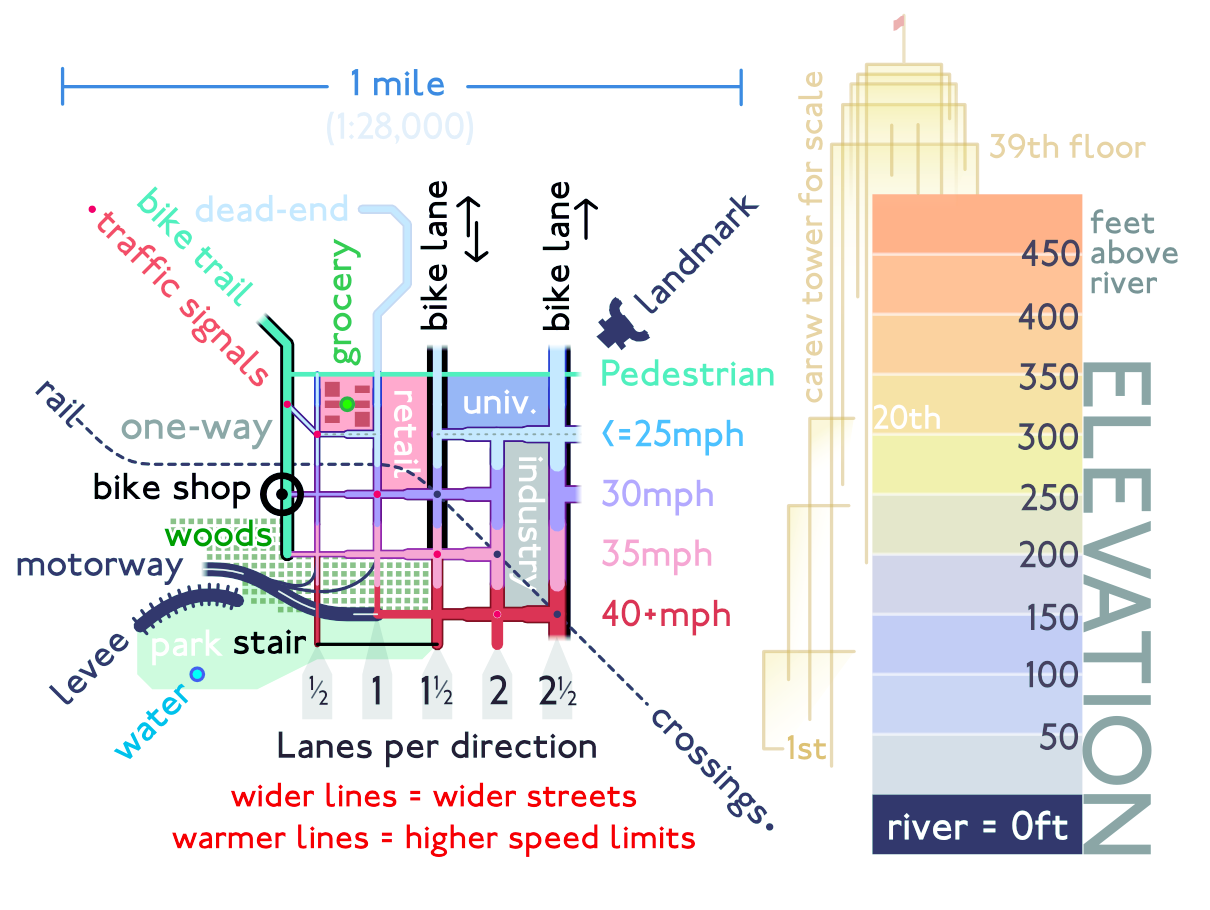
\includegraphics[width=0.4\textwidth]{legend}
			\caption{From the legend of the Cincinnati Bike Map.}
			\label{fig:legend}
		\end{figure}
		
		Cincinnati has quite a few cul-de-sacs and the way these have been handled on signs and maps has always bothered me just a bit. A dead-end for a car may not be a dead-end for a bike or a pedestrian and indeed it very often isn't.
		One of the more innovative ideas I had in working on the map was to algorithmically detect dead-ends from a cyclist's perspective so that they could be de-emphasized relative to other streets.\footnote{
			Tarjan's algorithm for the detection of strongly connected subcomponents. Any edge not belonging to the main strongly connected component was rendered partly transparent.
		} This greatly reduced visual noise in some areas and helped the eye to follow through-streets where they existed.
		This cycling-specific measure of network connectivity ended up rather dramatically improving the readability of the map. 
		
		I eventually printed and distributed the map (9,000 paper copies and online) with the help of a local foundation and several generous sponsors. The project is described in much greater detail in an article in Cartographic Perspectives which is available online.\footnote{\fullcite{Wessel2015}}
	
	\section*{Lessons learned}
		Over the next year or so as I used my new map more and more for actual navigation, I began to wonder if there weren't a better way of doing things. By mapping road width onto the width of lines on the map (See Figure \ref{fig:legend}), I had retained something of the standard car-centric perspective: bigger streets with more lanes for cars were generally bigger and bolder on my map, regardless of their utility for cyclists. The algorithm I used to find dead-ends had some annoying limitations as well.
		
		It eventually hit me that I could kill these two birds with one stone. By simulating a huge number of cycling trips across the street network, I could estimate the relative importance of every street and path for cyclists, and at the same time deemphasize the dead-ends which implicitly are not useful for most trips.
		I found a realistic bicycle trip-planner\footnote{The Open Source Routing Machine or OSRM.} based on OpenStreetMap data for the travel simulation and got to work. 
		The measure I produced was similar conceptually to the problem of traffic assignment in transport modelling (i.e where congestion is not considered), or to the concept of betweenness centrality in graph theory.
		The results I produced were extremely interesting though life quickly got in the way of my progress: I graduated, moved to Toronto, and got too distracted by other work.
		
	\section*{A bike map for Toronto}
		The basic idea for this map has been simmering for several years now. I want to map a measure of usefulness or \textit{betweenness} onto the visual hierarchy of streets on the map. Bigger bolder lines will be streets that are more `useful' for cyclists, streets that would be used for more trips by bike. The measure will be influenced surely by the presence of bike lanes for example, but these won't be the only factor. It also matters where a street is in the broader network and what it connects. Bike lanes to nowhere will not distract us, and critical connections on unmarked service roads will stand out like they should. 
		
		For example if we have a street with a long, useful bike lane, but that lane has gaps and discontinuities, we may see that the segments connecting the portions with bike lanes are just as important to the cyclist because the street \textit{as a whole} serves a useful role in the network. 
		Presenting a continuous visual hierarchy to the reader should make the network easier to read, navigate, and remember.\footnote{
			This is a supposition which I nearly examined empirically as the topic of my dissertation research - I even developed software for the user study though ultimately took my research in a different direction.
		} 
		
		The map on the next page illustrates this more clearly. 
		
		This is illustrated in Figure \ref{fig:spanned-gap} where the algorithm picks up an important connection between the bike lanes on Lansdowne Avenue and The Queensway. 
		
		\begin{figure}[h!]
			\centering
			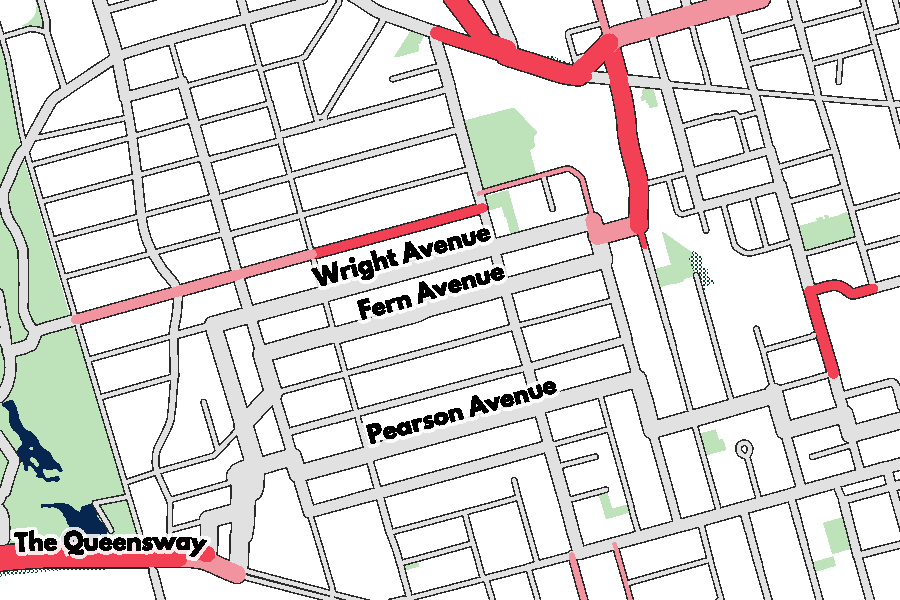
\includegraphics[width=0.45\textwidth]{spanned-gap}
			\caption{Wright, Fern, and Pearson Avenues are shown to be important connectors despite their lack of {\color{red}bike lanes}.}
			\label{fig:spanned-gap}
		\end{figure}
	
	\section*{What remains to be done}
		A prototype of the map is complete - a proof of concept. In order to produce a high-quality finished map, I need funding to complete the work.
		There is a great deal of manual data cleaning, surveying and verification that must happen to ensure quality. I need to fully localize the bicycle trip simulation to the particulars of Toronto. I need to create and apply a cartographic simplification and generalization algorithm to the input data. I need to engage local cyclists to validate the map against their experiences. Finally, I need to produce a complete print layout, find a printer, and produce and help to distribute thousands of maps in person and online. 
	
\end{document}